\documentclass{article}
\usepackage{graphicx}
\usepackage{tocloft} 
\usepackage{glossaries}
\usepackage{lipsum}
\usepackage{geometry}
\usepackage{fancyhdr} 
\usepackage{amsmath}
\usepackage{biblatex}  

\addbibresource{./common/references.bib}  

\geometry{a4paper, margin= 1in}

\makeglossaries
\loadglsentries{./common/glossary}

\title{Software Requirement Specification (SRS)}
\author{Group 1 }
\date{November 29 2024}

\begin{document}
\maketitle  
\pagebreak

\tableofcontents
\pagebreak

\section*{Version History}
\begin{longtable}{|c|c|p{10cm}|}
\hline
\textbf{Version} & \textbf{Date} & \textbf{Description} \\ \hline
4.0 & \today & Filled out the 2.1 and 2.2 section \\ \hline
\end{longtable}
\pagebreak


\includegraphics[width=0.3\linewidth]{./logo/csula.png} 

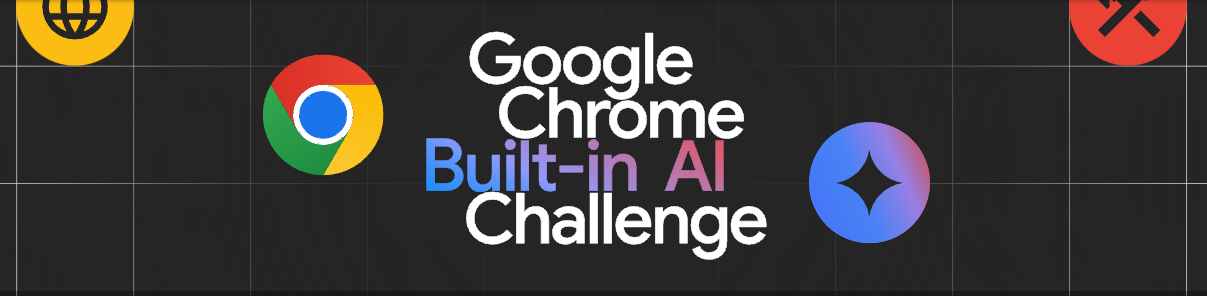
\includegraphics[width=0.3\linewidth]{./logo/chromeai.png} 

\section{Introduction}
\subsection{Purpose}
The purpose of this project is to describe the detailed requirements and design considerations for our project, "Google Chrome Built-in \Gls{ai} Challenge", available at \url{https://googlechromeai.devpost.com/}.

The project aims to use Chrome's built-in AI APIs and integrate functionalities powered by AI models such as Gemini Nano, with the goal of developing a web application or Chrome Extension that's able to interact with these APIs in order to offer features like dynamic prompt generation, summarization of text, multilingual translation, and text rewriting.

As for this Software Requirements Specification (SRS), its goal is to serve as a comprehensive guide for stakeholders, developers, and testers. It defines the functional and non-functional requirements, user interface specifications, and the system architecture in order to ensure a successful implementation of this project.

\subsection{Intended Audience}
The intended audience for this document includes:
\begin{itemize}
    \item \textbf{Developers:} So that they can understand the technical specifications and requirements necessary to integrate the needed APIs into a functional web application or extension. 
    \item \textbf{Testers:} So that they can use this document to understand the functional requirements and design considerations. They'll need that in order to create and execute test cases to help validate the application’s features, ensuring that it meets the defined requirements.
    \item \textbf{Stakeholders:} So that they can ensure that the project aligns with the goals of the challenge, evaluating its feasibility, business value, and compliance with technical and operational constraints.
\end{itemize}

This document assumes that the audience has a general understanding of software engineering principles, AI technologies, and Chrome Extension development.

\subsection{Overview of the Software}
 The project is the development of a Chrome Extension or web application that uses Chrome’s built-in Artificial Intelligence (Ai) APIs to integrate with other AI models. The main features of the software include:

\begin{itemize}
    \item \textbf{Dynamic Prompt Generation:} By using the Prompt API, the application allows users to dynamically create prompts based on their input, which enhances the interaction experience with the AI models.
    \item \textbf{Summarization:} By using the Summarization API, the program will be able to condense large amounts of text into concise summaries, giving users clear insights from lengthy documents or articles.
    \item \textbf{Multilingual Translation:}By using Translation API, users will be able to translate content into multiple languages, allowing for there to be accessibility and usability for diverse audiences.
    \item \textbf{Text Rewriting:} By using the Rewrite API, alternative wordings or rephrases for the text will be suggested to the user in order for there to be better clarity or readability.
\end{itemize}

This project serves as a guide for how to approach the integration of AI-driven browser-based applications by using Chrome’s built-in capabilities. The goal is to build a user-friendly and efficient tool that empowers users to harness AI for everyday tasks without the need for server-side interactions.

\section{External Interface Requirement}
\subsection{User Interface}
The user interface (UI) is designed to be intuitive and accessible, allowing for seamless interaction with the web application and the Chrome Extension. Some of the main components of the UI are:

\begin{itemize}
    \item \textbf{Main Dashboard:} The main area where the users can access the core functionalities, like prompt generation, text summarization, multilingual translation, and text rewriting. Each of these features will be represented by an icon or button for easy navigation.
    \item \textbf{Prompt Input Box:} A text field where users will be able to input their queries or instructions. This box will support dynamic prompts as well as suggestions in case of misspellings or any other issues.
    \item \textbf{Summarization Panel:} A section of the page where the users can either type, paste, or upload whatever text they'd like to be summarized. The results will be displayed in another text box under this one in a clear and concise format, while the original text remains there to allow for comparison.
    \item \textbf{Translation Tool:} Another section of the page where the user can input their text and then select the language they'd like to translate to from a menu. While the program should automatically detect the language received, there's also an option to manually select what language is inputted. The translated text will be displayed instantly below the input box.
    \item \textbf{Rewrite Suggestions Panel:} A side panel that displays alternative wordings or rephrased versions of what the user inputted. Users can select their preferred rewrite or choose to stick to what they wrote..
    \item \textbf{Navigation Bar:} A menu bar located at the top of the application that will always be there no matter what, offering links to settings, user guides, feedback, and account management.
\end{itemize}

The UI will offer some tools and options including high-contrast mode, keyboard navigation, and screen reader support, improving usability for all users.

\subsection{Software Interface}
The software interfaces allow for communication between the application and the built-in AI APIs, with some key interactions being:

\begin{itemize}
    \item \textbf{Prompt API:} 
    \begin{itemize}
        \item Input: User-provided text prompts or questions.
        \item Output: Real-time suggestions and responses based on the user's input.
        \item Communication: Uses JavaScript to send requests directly to the built-in Prompt API for processing.
    \end{itemize}
    
    \item \textbf{Summarization API:}
    \begin{itemize}
        \item Input: Text content or uploaded documents.
        \item Output: Condensed summaries highlighting the most important elements of the inputted text.
        \item Communication: The application passes text data to the Summarization API, and the results are rendered in the Summarization Panel.
    \end{itemize}
    
    \item \textbf{Translation API:}
    \begin{itemize}
        \item Input: Source text and selected language.
        \item Output: Translated text in the target language.
        \item Communication: The application invokes the Translation API with language parameters and renders the results in the Translation Tool interface.
    \end{itemize}

\item \textbf{Rewrite API:}
    \begin{itemize}
        \item Input: User-provided text.
        \item Output: Alternative wordings, rephrased sentences, fixed spellings.
        \item Communication: Text data is sent to the Rewrite API, and suggestions are displayed in the Rewrite Suggestions Panel.
    \end{itemize}
\end{itemize}

The APIs are integrated directly into Chrome, which means can be accessed locally within the browser environment. This eliminates the need for external server calls, ensuring privacy and enhanced performance.

\section{Legal and Ethical Considerations}
\subsection{Data Storage and Privacy Considerations}
For our application, all interactions will occur within the local browser environment (Google Chrome). Here are a couple of considerations we'd like to address:
\begin{itemize}
    \item All user data will be securely processed within the browser. There will not be any form of external logging or monitoring on our user's activity.
    \item User sensitive data will be encrypted.
    \item Any cached data in use will be cleared once the application is closed, no sensitive information will be left on the user’s device.
    \item Our application will abide by regulations such as the General Data Protection Regulation (GDPR) and the California Consumer Privacy Act (CCPA). This means that the user is in control over both their privacy and personal data.
\end{itemize}
Our users will all be explicitly informed about how their data is handled and before our application starts processing information, we will explicitly ask the user for their consent.

\subsection{Possible Legal or Ethical Issues}
A couple of potential legal and ethical concerns to take note of and address for our applicafion:
\begin{itemize}
    \item \textbf{Data Minimization:} Our software shall collect only the data necessary for it to function properly. User input data will not be stored longer than required unless granted permission or explicitly requested by the user.
    \item \textbf{User Consent for Data Usage:} Users will be fully informed about how their data will be processed. They will have the ability to opt-in for data collection features such as saving input history or sharing data with third-party services.
    \item \textbf{Artificial Intelligence Biases:} Due to our application being integrated with Gemini Nano, users must be wary that AI models such as ours may produce biased or incorrect results. Misunderstanding of this information could lead to misinformation or unintentional harm. It is our duty and responsibility to provide our users with clear disclaimers regarding the limitations and capabilities of Gemini Nano.
    \item \textbf{Intellectual Property:} It is possible for our users to input copyrighted material into the our tools for summarization or rewriting. To avoid such legal issues, we will provide an explicit disclaimer informing users that they will be solely responsible for ensuring compliance with copyright laws.
    \item \textbf{Licensing Compliance:} Adhering to the terms and conditions of the AI API providers is essential. Misuse of APIs could result in license revocation or legal disputes.
\end{itemize}
Ethical guidelines will be strictly enforced to ensure that the our application prioritizes the safety of our users and complies with all relevant laws and standards.

\section{Glossary}
\begin{longtable}{|p{3cm}|p{10cm}|}
\hline
\textbf{Acronym} & \textbf{Definition} \\ \hline
AI & Artificial Intelligence: Simulating human intelligence in machines to perform tasks like learning, reasoning, and self-correction. \\ \hline
API & Application Programming Interface: A set of functions and protocols that allow different software applications to communicate. \\ \hline
CCPA & California Consumer Privacy Act: A California law that provides data privacy rights and protections for residents of California. \\ \hline
GDPR & General Data Protection Regulation: A regulation in EU law on data protection and privacy in the European Union and the European Economic Area. \\ \hline
SRS & Software Requirements Specification: A document that outlines the functional and non-functional requirements of a software application. \\ \hline
UI & User Interface: The visual and interactive part of an application where users interact with the system. \\ \hline
\end{longtable}

\printglossaries
\end{document}